\chapter{Basic operations} \label{chap:basicop}

    \vspace{-1cm}
    \section{Introduction} 
    \vspace{-0.7cm}
This chapter introduces some of the most basic ingredients of computer programming 
using its foundational concepts of mathematics.
Data types, data structures, maths operators, etc.
find their origins in mathematical objects.
In a given branch of mathematics, an object is anything that can be formally defined and 
which is subject of deductive reasoning. 
For example, the numbers are objects in the Numbers Theory and
all algebraic structures are objects in Abstract Algebra.
But first let's give some context. 

An \textbf{algorithm} in mathematics is a finite and ordered sequence of unambiguous instructions to solve a specific problem. 
Notice that this definition involves that i) the algorithm ends in a finite number of steps, 
ii) the sequence of instructions that yields the output are followed in their numerical order and
iii) inputs, instructions and outputs must be properly identified. 

The \textbf{problem} to solve can be seen as a function between a bunch of inputs and their associated outputs.
The algorithm solves and instance of this function, which means, its particularization on a specific set of inputs.
Given a problem, an algorithm to solve it and a machine, 
the \textbf{theory of computation} gives the basis for the automatic processing of the algorithm
and answers things like how efficiently the problem is solved. 

To use \textbf{machines} we need to speak their language.
The \textbf{program} or code is the translation of the algorithm (mathematical language) 
to a language understood by the machine, the programming language. 
Hence, 
an algorithm breaks down a complex problem into simpler instructions 
and then is translated into a program so the machine can understand it. 
Most programming languages have the same components as building blocks to translate these instructions:
\begin{itemize}[noitemsep]
    \item \textbf{Statements and Expressions:} Statements are all line of code that instructs the compiler to perform a task.
    There are several types of statements like assignments, procedures calls, input/output statements or control flow structures. 
    It is usually distinguished between statement and expression. 
    The former is executed with no value as a result, only a compiler instruction, 
    the latter is evaluated and ends with a resulting value.
    \begin{itemize}
        \item \textbf{Control flow structures:} These are the structures that, by means of keywords, allow to control the flow of data along the program. 
        The most basic control structures are the loops, which let instructions be repeated until a condition is reached and 
        the conditionals, which allow to make decisions and execute instructions accordingly.  
    \end{itemize}
    
    \item \textbf{Variables and Data structures:} A variable involves a tag that identifies a memory location and 
    the content of the memory, the data itself. 
    This attached data, of different types (integer, real, character, etc.), may change during the execution of the program.
    In contrast, \textbf{constants} may also have a name but the data don't change during the execution.
    Data structures are also used to store, organize and process data, 
    now arranged in a specific way so that it can be treated efficiently. 
    Some common data structures are arrays, sets, lists, tuples, trees, graphs, etc.
    
    \item \textbf{Operators:} Symbols that tell the compiler to perform operations of different kind in order to produce a result.
    There are arithmetic operators ($+$, $*$, $-$, $/$, etc.), 
    relational ($>$, $<$, $==$, etc.), 
    logical operators (\texttt{AND}, \texttt{OR}, \texttt{NOT}), etc. 
    Sometimes the assignment operator (\texttt{=}) is also included in this classification, 
    however, it has a different nature. 
    
    \item \textbf{Functions, Procedures:} Procedures and functions in computer science are usually defined as 
    named blocks of code that are called to perform a task, maybe accepting some input arguments and maybe returning some output values. 
    Pure functions can be included here, the representation of the mathematical functions in programming. 
    
    \item \textbf{Objects:} objects are constructions with 
    \textit{state} (combinations of variables and data structures) and 
    \textit{behaviour} (combinations of functions and methods) 
    to represent concepts and objects of the real world. 
    A complex number could be an object, 
    whose state needs from variables: the real and imaginary parts, and 
    whose behaviour involves addition, multiplication, conjugation among others. 
    
    \item \textbf{Comments:} Lines of code intended to help programmers understand the code, 
    but which are not read or executed by the compiler.
\end{itemize}
\vspace{-0.5cm}
Other \textbf{keywords and characters} are usually reserved by each programming language 
in order to perform tasks like: 
group expressions (parenthesis), 
delimit characters (\texttt{''}), 
break lines of code, 
include more than one statement in a line, etc.

Finally, the \textbf{compiler/interpreter directives} are not part of the programming language itself 
but also instructs the compiler to perform tasks. 
These statements cause the compiler to take a specific action during compilation and 
may vary from compiler to compiler.


Let's see all these components together, 
do not worry if the syntax of the languages or 
the meaning of the keywords are not clear at this point. 
The first example solves the roots of a second degree equation in Fortran and 
the other example reads real and imaginary parts of a complex number with Python.

\begin{figure}[h]
    \centering
    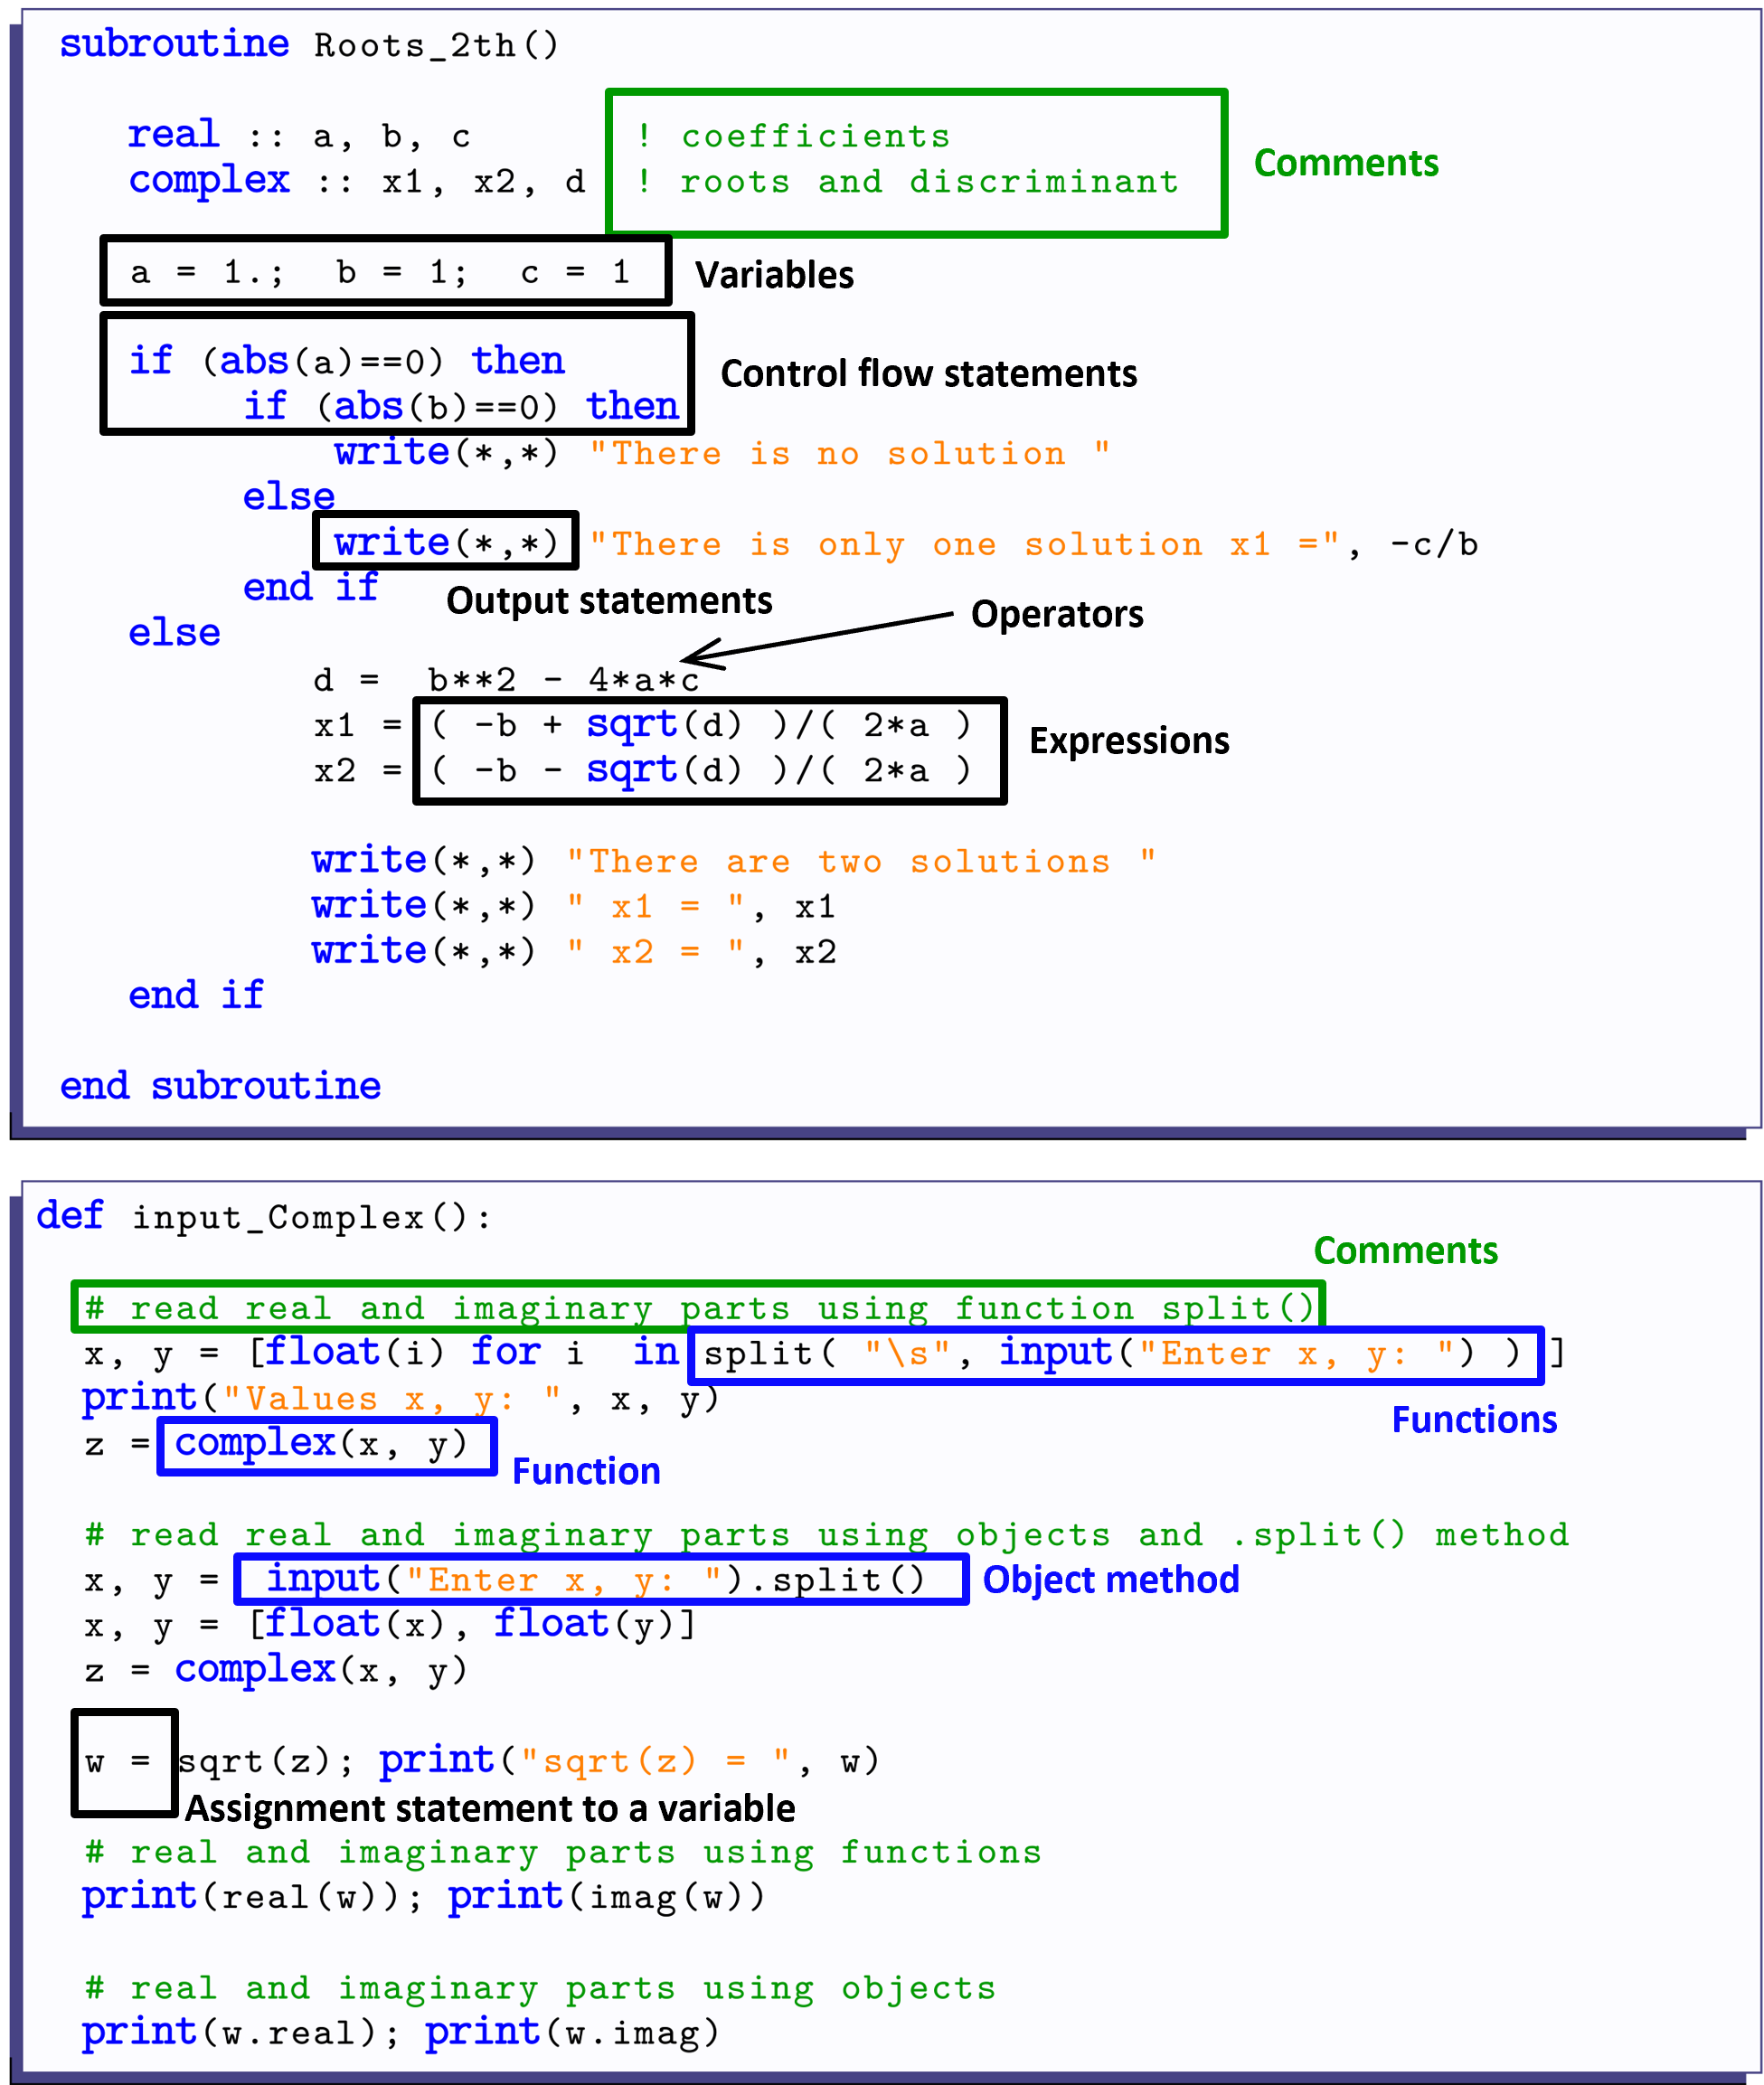
\includegraphics[width=.95\textwidth]{./doc/Figures/components.png}
    \caption{Main building blocks used to code in common programming languages.}
    \label{fig:components}
\end{figure}
\FloatBarrier
%THIS CODE IS USED TO GENERATE LATER THE IMAGE...
%\vspace{0.5cm}
%\renewcommand{\home}{./Fortran/sources/Foundations/Roots} 
%\lstfor
%\listings{\home/Roots.f90}{subroutine Roots_2th}{end subroutine}{}
%
%\renewcommand{\home}{./Python/sources/Foundations/Data_type} 
%\lstpython
%\listingsp{\home/data_type.py}{def input_Complex}{w.imag}{}


 
 
 
 
 
 
 



%MORE:
%Input: getting data and commands into the computer
%Output: getting your results out of the computer

%Libro FORTRAN: Programación Multicapa

%Most important basic elements for programming languages are:
%Programming Environment
%Keywords
%Input and Output Operations

%Functions
%A function is a statement that returns a value. For example, the function InputBox() returns the value of its dialog text field.
%Objects
%An object is a program “building block” entity. It can be visible, like a Button control, or invisible like a Timer control.
%Properties
%A property is a characteristic of an object. For example, the property Btn.Text is the Text property of the Btn object.
%Methods
%A method is an action that an object can perform. For example, the method Btn.Click() is the Click method of the Btn object.



%The assignment statement \texttt{v = 3*5 + 2} becomes the bottleneck of programming languages in the sense that a program is mainly concerned 
%with the flow of assignments of single variables (imitating single words). 
%By executing assignments many times, maybe altering subscripts (imitating memory addresses), 
%the program ends up with the result stored in a variable (imitating the storage in memory). 
%Furthermore, this assignment statement splits the programming languages into two worlds: 
%a world of expressions with strong algebraic properties (\texttt{3*5 + 2}) and a world of statements with few mathematical properties (\texttt{v =}).




    \section{Data types}
    
Several objects are used to build the different branches of mathematics; numbers, operations, functions, sets, vectors, matrices, tensors and a large etcetera. 
Let's review here the formal definition of some objects that later are represented in programming by means of the data types. 

In mathematics, the numbers are usually classified into sets according to their nature.
The set of integers $\mathbb{Z}$ includes the number zero (0), the natural numbers ($\mathbb{N} = \{ 1,2,3,... \}$) and their additive inverses, the negative numbers ($\{ -1,-2,-3,... \}$).
The set of real numbers ($\mathbb{R}$) includes any number identified with a point on the real number line.
$\mathbb{R}$ includes both the set of rational numbers ($\mathbb{Q}$) and the set of irrational numbers.
Finally, the complex numbers ($\mathbb{C}$) extends the real numbers using the imaginary unit, an element satisfying the equation $i^2 = -1$, which does not have solution among the reals.
Once introduced the imaginary unit, every complex number can be expressed as $a+bi$ where $a,b\in\mathbb{R}$. 

The fact that a number belongs to one or another set is not only important from the classification point of view.
It also comes with a long list of derived consequences which are essential to build mathematics. 
Let's take for example $\mathbb{Z}$ equipped with the usual addition, multiplication and ordering. 
Automatically we can assert that for any $a,b\in\mathbb{Z}$, $a\cdot b\in\mathbb{Z}$ and $a+b\in\mathbb{Z}$.
Also, we do not have to worry about the order to operate them since $a+b=b+a$ and $a\cdot b = b\cdot a$.
To mention other results, for $a,b>0$ then $a+b>0$, $a+b>a$, $a+b>b$, $a\cdot b>0$, $a\cdot b\geq a$, $a\cdot b\geq b$, the equation $a+x = 0$ has a unique solution $x\in\mathbb{Z}$, etc.

Some properties are based on others until a whole theory around the integers is built. 
The same happens with $\mathbb{N}$, $\mathbb{R}$, $\mathbb{C}$, etc. 
When these mathematical objects are used in a computer, 
we are not only using some specific values (elements of the set) but also
all the properties and results attached to them. 

Jumping to a different context like the Boolean algebra, the same principle applies.
However, now the elements to consider are the truth values: \textit{true} and \textit{false}, instead of numbers.
Also, the basic operations between these elements are conjunction (and), disjunction (or) and negation (not) 
instead of binary operations like addition and multiplication.

Hence, each constant, variable, array or function in a programming language has an intrinsic data type associated, 
said in other words, a set to which they belong. 
This type decides, among other things, the allowed values that the entity can have and the set of operations that can be performed with them.
For example, the set of integers in mathematics is represented in a programming language through \texttt{integer} data type. 
Then, a value $i\in\mathbb{Z}$ will be stored in an \texttt{integer} variable that admits addition, multiplication or exponentiation.


        \newpage
        \subsection*{Fortran code}
Fortran provides five intrinsic data types. 
Derived data types can be created either from intrinsic types or from other derived types previously defined.
The code below shows the declaration and initialization of the five intrinsic data types, which are:
\begin{itemize}
    \item Numeric nature: \texttt{integer}, \texttt{real}, \texttt{complex}. 
    \item Boolean nature: \texttt{logical}.
    \item Text nature: \texttt{character}.
\end{itemize}
Roughly speaking, a value $n\in \mathbb{Z}$ is stored in an \texttt{integer}, 
$x\in \mathbb{R}$ is stored in a \texttt{real} and 
$z\in \mathbb{C}$ is stored in a \texttt{complex} variable.
Many nuances to the equivalence between the programming concept and the mathematical abstraction 
for integers and reals are treated in the Part \ref{PartII} of this book. 

The \texttt{logical} type gets the two possible values of the Boolean algebra; \texttt{True} and \texttt{False}. 
Finally, the \texttt{character} type can store strings with ASCII characters which includes alphanumeric, symbols and sign characters.   
\vspace{0.5cm}
\lstfor
\renewcommand{\home}{./Fortran/sources/Foundations/Basic operations} 
\listings{\home/Basic_operations.f90}{subroutine Data_types}
{end subroutine}{Basic_operations.f90}

The data typing in a programming language is \textbf{explicit} when the programmer needs to decide and declare the type for each variable or \textbf{implicit} when the language assumes it. 
Furthermore, while some programming languages allow the use of some data types as if they were a different type (weak typing) others does not (strong typing). 
Since Fortran is an explicit typing language, before using any variable, all must be previously declared with a specific type.

 



        \newpage 
        \subsection*{Python code}
The same five data types, also known as primitive data types, are built-in in Python but with a different name.
In addition, Python also allows non-primitive data types (explained in this book as data structures)
and user-defined data structures.
\begin{itemize}
    \item Numeric nature: \texttt{int}, \texttt{float}, \texttt{complex}. 
    \item Boolean nature: \texttt{bool}.
    \item Text nature: \texttt{str}.
\end{itemize}

Since Python is mainly an implicit typing language notice that we don't declare the type of any variable and just initialize it.
The following program shows an example of the initialization of the five data types we can find. 
\vspace{0.5cm} 
\renewcommand{\home}{./Python/sources/Foundations/Data_type} 
\lstpython
\listingsp{\home/data_type.py}{def data_types}
{string}{data_type.py}


    \newpage
    \section{Data structures} 
\vspace{-0.5cm}
Numbers and truth values are not the only objects needed to build the different branches of mathematics.
Also sets, vectors, tuples, matrices, tensors or sequences are used in the context of algebra, calculus or set theory.
Let's review now the formal definition of the objects that later are represented in programming by arrays, sets, tuples and lists. 

%set --------------------------------------------------------------
A \textbf{set}, with the definition given by Georg Cantor within the set theory, 
is a gathering together into a whole of definite, distinct objects of our perception or our thought, 
which are called elements of the set.
The elements of a set can be any mathematical objects: numbers, points in space, geometrical shapes, variables or other sets.
However, every element of the set must be different from the others.

Let's create as an example the set of the prime numbers up to 50:
$$
\{2, 3, 5, 7, 11, 13, 17, 19, 23, 29, 31, 37, 41, 43, 47, 53, 59, 61, 67, 71, 73, 79, 83, 89, 97\}
$$

% --------------------------------------------------------------

Tuples and sequences are also collections of mathematical objects.
However, a \textbf{sequence} is an enumerated collection, where repetitions are allowed and order matters.
Unlike sets, since the elements follow an order, they can be repeated in different positions of the sequence.
A sequence can also be interpreted (and it usually is) as a function whose domain is a countably ordered set like $\mathbb{N}$ 
(denoting the position within the sequence) to the set of elements.
The length of the sequence is its number of elements and could be any finite value (like in the sequence $(1,5,6,5,8,10)$) 
or infinite (like Fibonacci sequence). 
Sequences are essential in different branches of mathematics, specially in analysis since they are 
the basis for series.

Notice that sequences are not defined in terms of vectors in any sense. 
It can happen that a sequence with elements in a field $\mathbb{F}$ 
(whether finite or infinite)
is a vector in the vector space of all sequences with elements in $\mathbb{F}$.
This is because the addition and multiplication by scalars in $\mathbb{F}$ 
can be defined in terms element wise common addition and multiplication, 
and satisfy the vector axioms, hence, we have a space vector over $\mathbb{F}$.
However, there is no need that the elements belong to a field and hence, no need 
to consider sequences as vectors. 

Let's find in the examples below an approximation to the infinite sum of the sequence: 
$$
\left[\sqrt{\frac{n}{n^4+1}}| n\in\mathbb{N}\right]
$$


% --------------------------------------------------------------

A \textbf{tuple} is a finite sequence, which means, a finite ordered lists of elements. 
It is usually used the notation $n-$tuple for a list of $n$ elements, where $n$ is a non-negative integer.
Again, under certain conditions, tuples can be seen as vectors, in this case from finite dimensional vector spaces. 
However, since tuples does not need to have elements from a field, its definition is not based in vectors in any sense. 

As an example of tuple use let's generate a set of Pythagorean triples, 
tuples like $\left(a,b,c\in\mathbb{Z}^+|a^2 + b^2 = c^2\right)$ using the following three equations:
\begin{equation}
    \begin{cases}
        a  & = i^2 - 1\\
        b & = 2i\\
        c & = i^2+1
    \end{cases}       
\end{equation}

%--------------------------------------------------------------
%vectors
Historically the term vector was used for geometric vectors, objects that has magnitude and direction.
However, a \textbf{vector} is any element of a vector space. 
Hence, members of a set that can be added together and multiplied by numbers of a given field, satisfying some axioms.

These vector spaces can be finite dimensional like the commonly used $\mathbb{F}^{n}$ 
(where $\mathbb{F}$ is a field like for example $\mathbb{R}$ or $\mathbb{C}$).
In these cases, $n-$tuples with elements in the field $\mathbb{F}$ are usually used to represent the vectors once a basis has been chosen. 
Hence, tuples are used to represent the vectors in a specific basis but not being the vectors themselves.
As an example, $\mathbb{R}^{2}$ or $\mathbb{R}^{3}$ are vector spaces 
usually represented as 2-tuples and 3-tuples of reals with respect to a given basis.
When $n-$tuples are used to represent the vectors we can use a one-dimensional arrangement of $n$ elements.

Vector spaces can also be infinite dimensional, for example the vector space of infinite sequences of real numbers $\mathbb{R}^\infty$ or 
the set of all continuous real valued functions on $[0,1]$. Now tuples cannot be used to represent vectors and sequences sometimes can.
It is clear then that some vectors could be seen as tuples, or sequences, but again there is no need to define 
vectors in terms of these objects since it is not the general situation. 

A \textbf{matrix} is a rectangular arrangement of numbers (or other mathematical objects) distributed in rows and columns.
Matrices over a field $\mathbb{F}$ are those where all its \textit{elements} or \textit{entries} belong to the field $\mathbb{F}$.
If $\mathbb{F}$ is $\mathbb{R}$ or $\mathbb{C}$ it conforms real matrices or complex matrices respectively.
It is usually used $\mathbb{F}^{n\times m}$ or ${\cal{M}}^{n \times m} (\mathbb{F})$ to denote 
the set of $n\times m$ matrices with entries in the field $\mathbb{F}$. 
This set, together with the common addition of matrices and the multiplication by numbers (scalars) 
in the field $\mathbb{F}$ also has the structure of vector space. 
Hence, some matrices are also vectors inherited from the vector space structure they present.

%Tensors are NOT the generalization of scalars, vectors and matrices (no indices, one index, two indices) to an arbitrary number of indices. 
The concept of \textbf{tensor} has different approaches. 
Avoiding the formal definition let's consider here that a tensor can be represented as a potentially multidimensional array.
The elements in this multidimensional array are called scalar components and are denoted by indices with their position in the array.

Finally, we have used the term \textbf{array} (or arrangement) three times: 
a potential representation for tuples or vectors, 
a representation of matrices and a representation for tensors. 
In maths, an array refers to an orderly arrangement of similar 
mathematical objects, hence, following a specific pattern.

The standard notation for all these objects are as indicated below:
\begin{itemize}
    \item Sets are usually indicated by listing its elements between curly brackets $\{\}$ separated by commas (roster notation): $\{\textrm{car, boat, plane}\}$
    \item Sequences and tuples are usually written between parenthesis $()$ or square brackets $[]$: $(1,3,5,7,...)$ %or angle brackets $\langle \rangle$: 
    \item In a similar way vectors are usually enclosed in parentheses $()$: $(1,2,3,4,5)$ %or angle brackets $\langle \rangle$:  or $\langle1,2,3,4,5 \rangle$
    \item Matrices are commonly written with square brackets: %or parentheses:
    $
    \begin{bmatrix}
        1 & 2 & 3 \\
        4 & 5 & 6
    \end{bmatrix} 
    $
%    $ or $
%    \begin{pmatrix}
%        1 & 2 & 3\\
%        4 & 5 & 6
%    \end{pmatrix}   
%    $
    \item A tensor is usually denoted by a symbolic name followed by a collection of subscripts where the number of subscripts attached defines the rank of the tensor.
    For example $\alpha_{ijkl}$ is a rank 4 tensor.
\end{itemize}
% -------------------------------------------------------------- 



In a programming language all these objects are represented by different data structures.
Fortran for example does not include tuples, sets or sequences, but vectors, matrices and tensors are represented with arrays. 
On the contrary, Python has built-in the structures of sets and tuples among others and arrays are available within the \texttt{NumPy} library.  

With the Fortran examples below the following concepts are covered:
\begin{enumerate}[noitemsep]
    \item Declaring arrays: type, rank and dimension.
    \item Initialize arrays: constructors. 
    \item Iterators for arrays, sectors or slices. 
\end{enumerate}

Also, with the Python examples, the following concepts are treated:
\begin{enumerate}[noitemsep]
    \item Constructors, iterators and slices for NumPy arrays.
    \item Using sets, lists, tuples and dictionaries: constructors.
    %\item Iterators for data structures.
\end{enumerate}





        \newpage
        \subsection*{Fortran code}
%Declaration
Consider the following vectors $V, W \in \mathbb{R}^N$, $X\in \mathbb{R}^6$, $Y\in \mathbb{R}^3$ and matrix $A \in { \cal{M}}^{N \times N} (\mathbb{R})$ 
with $N=10$ and let's declare them using Fortran arrays. 
$$
V = \left( v_i =\frac{1}{i^2} \right)^T, \quad W = \left( w_i = \frac{(-1)^{i+1}}{2i+1} \right)^T \;\; i = 1 \ldots  N,  \quad Y = \left(A_{i j}\right)_{\substack{i = 2 \\  3\leq j\leq 5}}^T
$$
$$
A = \left[ a_{ij} = \left( \frac{i}{N} \right)^{j-1}, \ \ i = 1 \ldots  N, \ \ j = 1 \ldots  N \right], \quad X = ( 1.3, 2.4, 3, 4.5, 5.3, 7 )^T
$$
An array, either representing a vector, a matrix or a tensor, is properly \textbf{declared} when it has 
type, rank and dimension (or extent) (see Figure \ref{fig:arrays}). 
The data type has already been treated before, in these examples we are using \texttt{real} vectors and matrices. 
The rank; the number of dimensions in the array, is 1 for column vectors, 2 for matrices and can be higher for higher dimension tensors.
The extent of each particular dimension is its length; the number of elements in that dimension.
\begin{IN}
Notice that, in Fortran, the \textbf{bounds of a dimension} may start with the index we prefer. 
By default it stars with index \texttt{1} but it can start in \texttt{0} or whatever index we want. 
For example the matrix \texttt{B(-2:4,0:1)} starts in \texttt{-2} and ends in \texttt{4} (also included) for the first dimension and 
\texttt{0} and \texttt{1} (also included) for the second dimension. 
\end{IN}
\vspace{0.5cm}
\lstfor
\renewcommand{\home}{./Fortran/sources/Foundations/Basic operations} 
\listings{\home/Basic_operations.f90}{subroutine Data_structures}
{4,0}{Basic_operations.f90}




%Initialization
Once declared, the \textbf{initialization} of the arrays is performed with constructors. 
Three ways are commonly used to manually construct an array: 
\vspace{-0.5cm}
\begin{enumerate}[noitemsep]
    \item \textbf{By a list of values:} \texttt{ [ list ] } where 'list' is a list of values of the same array type separated by commas. 
    For example the vector \texttt{X} in the code. 
    \item \textbf{Using an array expression:} \texttt{Y = [ A(2, 3:5) ]} stores the list of values in the second row of \texttt{A} from columns \texttt{3} to \texttt{5}.
    \item \textbf{Using an implicit loop:} a list of elements is computed from a loop. For example vectors \texttt{V}, \texttt{W} or matrix \texttt{A} in the code.
\end{enumerate}
In the case of Fortran the constructors are only used for rank-one arrays so 
functions like \texttt{reshape} are needed for higher ranks. 
For example the matrix \texttt{A} in the code is initialized using the \texttt{reshape} function.     
\vspace{0.2cm}
\lstfor
\renewcommand{\home}{./Fortran/sources/Foundations/Basic operations} 
\listings{\home/Basic_operations.f90}{1./i}
{2, 3}{Basic_operations.f90}    
    
   
  
    
%sectors, iterators... 
In Fortran the elements of the array are accessed using parenthesis notation and
an index in each dimension can be used as \textbf{iterator}.
This is intimately related to the \textbf{slicing}, for example the initialization of \texttt{Y} above use an slice of \texttt{A}.
This can also be extended to a whole dimension using the colon symbol, \texttt{C(:,2)} (see the example below and Figure \ref{fig:arrays}). 
Furthermore, alternate values can be selected by specifying a lower bound, an upper bound and the jump between values 
(see the example below and Figure \ref{fig:arrays}), \texttt{B(-2:4:3,:)} being the value \texttt{3} the jump between rows.
Notice that, since Fortran is a column major order language, functions like \texttt{reshape} and slicing treats the data by columns. 
\vspace{0.2cm}
\lstfor
\renewcommand{\home}{./Fortran/sources/Foundations/Basic operations} 
\listings{\home/Basic_operations.f90}{!Slices}
{end subroutine}{Basic_operations.f90} 

\begin{figure}
    \begin{subfigure}[b]{0.5\textwidth}
        \centering
        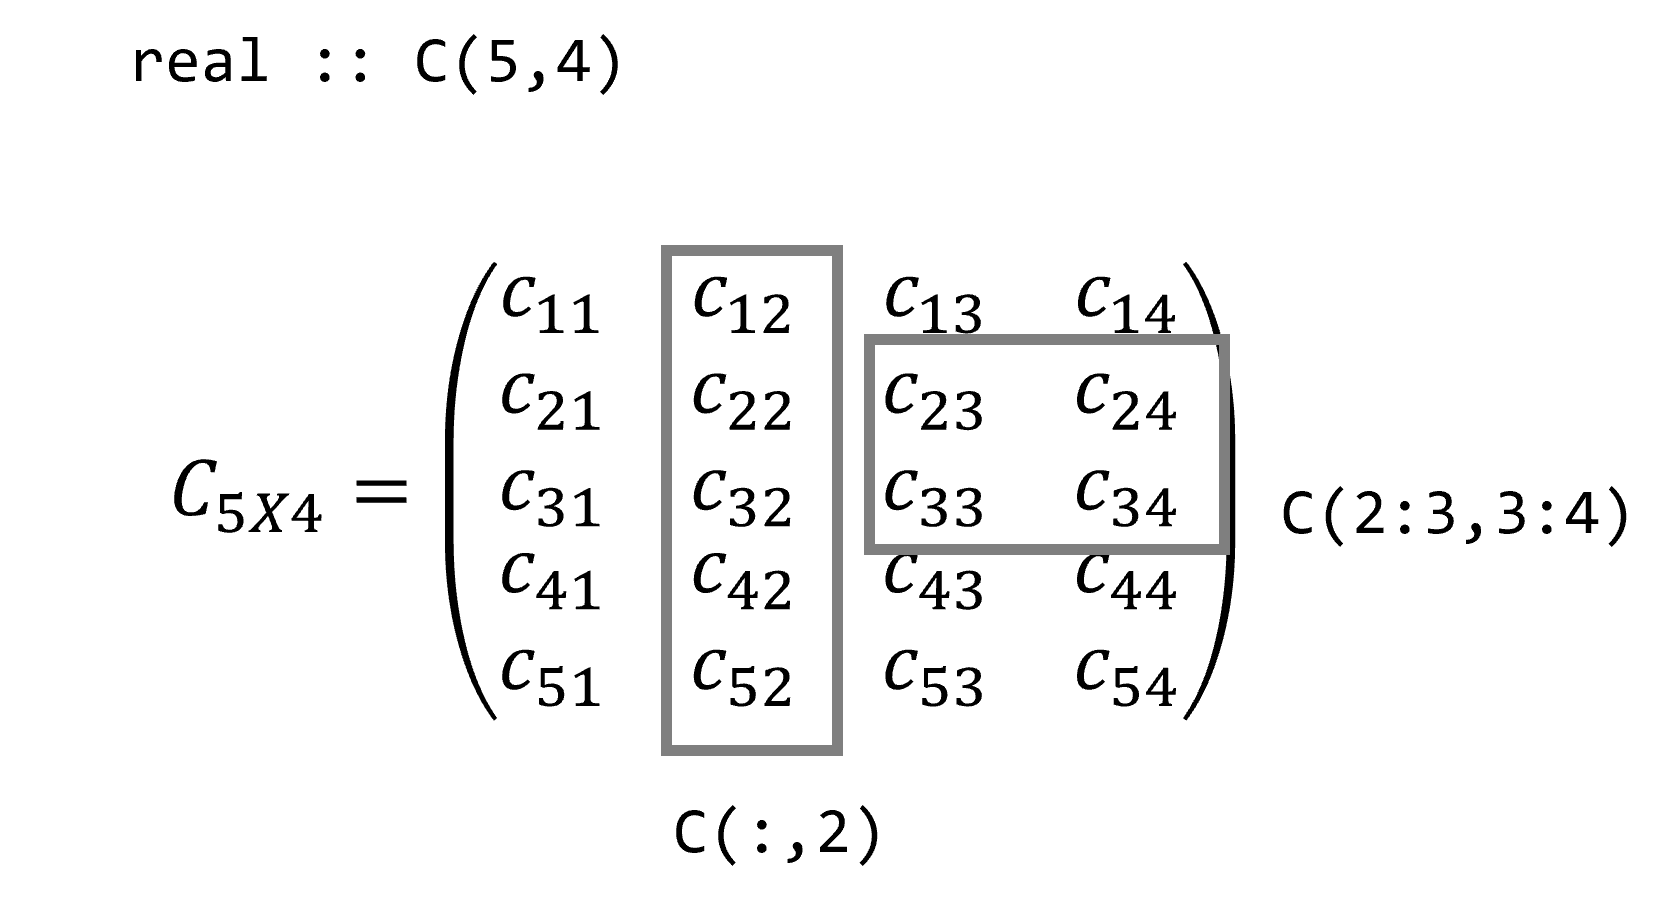
\includegraphics[width = \textwidth]{./doc/Figures/Array1.png}  \\
        \begin{center}
            Rank = 2 \\
            Extent = (5,4) \\
            Size = 20 \\
            Bounds = (1:5, 1:4) \\
            %Shape = (5, 4)
        \end{center}
    \end{subfigure}
    \hspace{\fill}
    \begin{subfigure}[b]{0.5\textwidth}
        \centering
        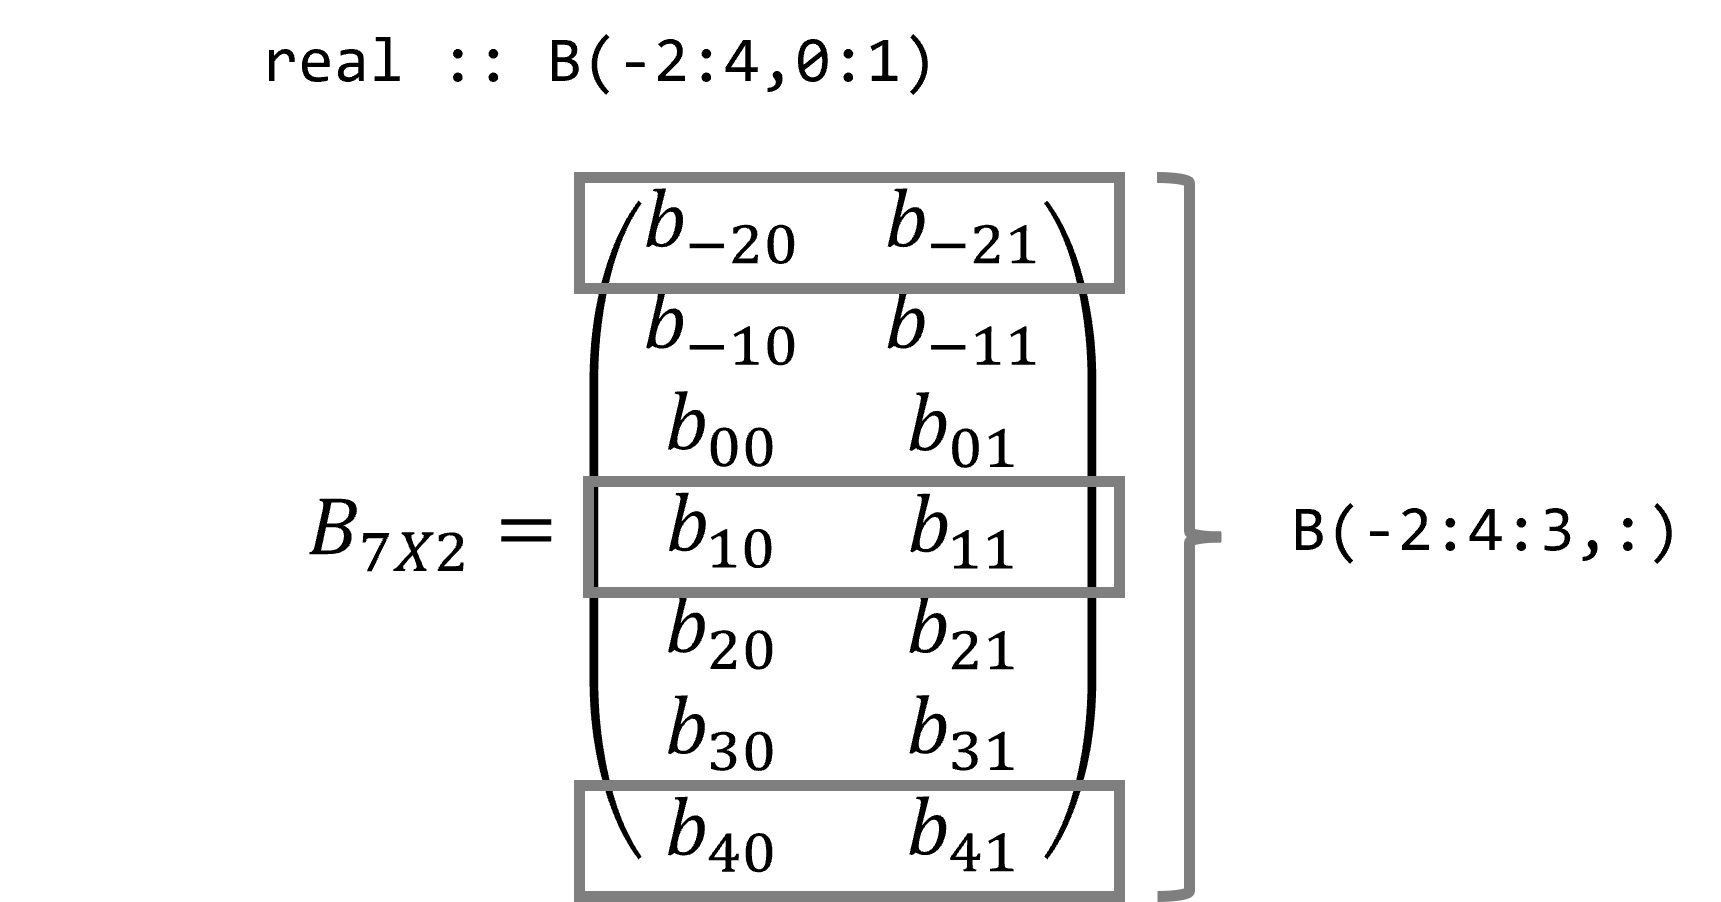
\includegraphics[width = \textwidth]{./doc/Figures/Array3.png}  \\
        \begin{center}
            Rank = 2 \\
            Extent = (7,2) \\
            Size = 14 \\
            Bounds = (-2:4, 0:1) \\
            %Shape = (7, 2)
        \end{center}
    \end{subfigure}
    \caption{Example arrays with their main properties.}   \label{fig:arrays}
\end{figure}







        \newpage 
        \subsection*{Python code}
Let's see the same examples defined above using \texttt{NumPy} arrays and 
let's include now a matrix $Z \in { \cal{M}}^{2 \times 3} (\mathbb{R})$. 
Notice that now they do not need to be explicitly declared, 
Python automatically does it. 
$$
Z =     
\begin{bmatrix}
    1.1 & 2.2 & 3.3\\
    4 & 5.6 & 6.2
\end{bmatrix} 
$$

%Initialization
The \textbf{initialization} of the arrays is performed using the \texttt{array()} function as constructor. 
Three ways are commonly used to manually construct an array: 
\begin{enumerate}[noitemsep]
    \item \textbf{By a list of values:} \texttt{ [ list ] } or \texttt{ [ [ list ], [ list ] ] } where \texttt{list} is a list of values of the same array type separated by commas. 
    For example the vector \texttt{X} or the matrix \texttt{Z}.
    Notice that Python allows manual constructors for higher than rank-one arrays.
    \item \textbf{Using an array expression:} \texttt{Y = A(1, 2:5)} stores the list of values in the second row of \texttt{A} from columns \texttt{3} to \texttt{5}.
    Notice that Python not only starts in \texttt{0} all the indices so \texttt{1} means the second column, 
    but also an slice like \texttt{2:5} ends in \texttt{4} so the slice takes columns \texttt{3} to \texttt{5}. 
    \item \textbf{Using an implicit loop (list comprehension):} a list of elements is computed from a loop. For example vectors \texttt{V}, \texttt{W} or matrix \texttt{A} in the code.
\end{enumerate}
%\vspace{0.5cm} 
\lstpython
\renewcommand{\home}{./Python/sources/Foundations/data_type} 
\listingsp{\home/data_type.py}{def arrays}{by rows}{data_type.py}

%sectors, iterators...    
In Python, the elements of the array are accessed using bracket notation, 
the array can be \textbf{iterated} using an index in each dimension and 
\textbf{slicing} is also allowed.
Notice here that NumPy arrays, contrary to Fortran, are row-major order. 
This means that arrays store the data by rows and then, in the previous example 
\texttt{C[1:3 ,2:4] = [ [1.,2.], [3.,4.] ]} will be assigned by rows. 

Similarly to Fortran, the colon symbol iterates in a whole dimension (see \texttt{C[:,1]} in the example above) and 
alternate values can be selected by specifying lower and upper bound and the jump between values.
However, the example \texttt{B(-2:4:3,:)} made with Fortran can not be copied because:
\begin{IN}
In Python, the \textbf{bounds of a dimension} always start with the index \texttt{0} (zero-indexing) and
stop 1 before the final bound.  
\end{IN}









\vspace{0.5cm}
Python has built-in other data structures which are used to store collections of data.
Their elements can be of any type for lists, tuples and dictionaries: 
strings together with integers and reals, 
lists nested in lists, tuples within lists, etc. 
Sets and ranges present some exceptions to consider in the elements they gather.
\vspace{-.5cm}
\begin{itemize}[noitemsep]    
    \item Set nature: \texttt{set}, \texttt{frozenset}.
    \item Sequence nature: \texttt{list}, \texttt{tuple}, \texttt{range}.
    \item Mapping nature: \texttt{dict}.
\end{itemize}
\vspace{-.5cm}

%--------------------------------------------------------------------------
A \texttt{set} in Python takes the same meaning as the mathematical object: a collection of any type of data that 
i) is unordered and 
ii) do not allow duplicate values. 
In a set, all that matters is whether each element is in it or not, so the ordering of the elements is irrelevant.
Furthermore, two equal elements, since they are not ordered, could not be distinguished between them. 
While a set is mutable (remove or add elements is allowed), a \texttt{frozenset} is an immutable set, once created, its content can not be modified. 
Sets cannot contain lists or dictionaries since they are unhashable structures (they do not contain any hash value that never changes during their lifetime).

%MATEMATICAS:
%List/Sequence: enumerated collection of objects in which repetitions are allowed and order matters. USUALLY INFINITE
%Tuple: enumerated collection of objects in which repetitions are allowed and order matters. ALWAYS FINITE

%PROGRAMMING PYTHON:
%List/Sequence: enumerated collection of objects in which repetitions are allowed and order matters. ONLY FINITE IS POSSIBLE
%Tuple: Same as list but it can not change (programming concept not related to maths)
A \texttt{list} extracts its meaning from the concept of sequence in mathematics,
however, in programming lists can not be infinite.
Hence, a list is characterised by being 
i) ordered: the position within the list is kept, 
ii) allow duplicates: items can appear more than one time in the list and  
iii) changeable: change, add, and remove items are allowed.
In a list, the difference between any two elements comes with the index within the list.
Notice that lists are not arrays or viceversa, in the sense that they come from completely different mathematical concepts. 

A \texttt{tuple} also takes the mathematical definition of tuple (a finite sequence). 
Since both tuples and lists are finite in the computer, the only difference between them are the changeability.
Hence, a tuple is characterised by being 
i) ordered: the position within the tuple is kept, 
ii) allow duplicates: items can appear more than one time in the tuple and  
iii) unchangeable: once created, it can not be modified.
For tuples, Python allocates the required memory once and not reallocates it. 
This becomes a more memory efficient strategy to follow when the data is going to be immutable.

A \texttt{range} structure is a sequence of integers that cannot produce the same number twice, 
it is strictly increasing or decreasing. 
This structure is more efficient than a list or tuple in the sense that only generates the values 
of the sequence when are needed and do not store any values in memory. 
Hence, they are efficiently used for loops.

A dictionary (\texttt{dict}) is similar to a list.
It is ordered, changeable and can store any type of data (even other dictionaries nested).
However, unlike lists, the values are stored in pairs: \texttt{key:value} and do not allow the same key for two elements.
%--------------------------------------------------------------------------



Let's now take a look at some examples of use cases of these structures. 
Notice that they do not need to be explicitly declared, 
Python automatically does it. 
The following notation is used to manually construct these structures: 
\vspace{-0.5cm}
\begin{itemize}[noitemsep]
    \item \textbf{Set:} Following the roster notation, it is defined by listing its elements between curly brackets and separated by commas.
    Notice that the sets \texttt{ \{``car'', 5, 6.7, 1 + 1j\} } and \texttt{\{5, 1 + 1j, 6.7, ``car'', 5\}} 
    are the same since repetition and order change do not modify it.
    Other example is the set \texttt{P} defined in the example below.
    \item \textbf{List:} Written using square brackets \texttt{[]} with comma-separated values. 
    Notice the sequence example of the summation of a sequence below.
    \item \textbf{Tuple:} Written using parenthesis \texttt{()} with comma-separated values. 
    For example the tuples defined in the set of Pythagorean triples.
    \item \textbf{Dictionary:} It has its list of elements separated by commas, 
    enclosed in curly brackets (\texttt{\{\}}) and 
    using a colon (\texttt{:}) to separate each pair. 
    Notice the example of dictionary below. 
    
    \item Sets, lists and tuples can be also defined using an \textbf{implicit loop (list comprehension)}, 
    the elements gathered in the structure are computed from a loop. 
    For example the set of Pythagorean tuples defined below.
\end{itemize}
\vspace{-0.5cm}
Notice that lists, tuples and dictionaries use the square brackets notation 
to access to their elements, similar to the NumPy arrays. 
\vspace{0.3cm} 
\lstpython
\renewcommand{\home}{./Python/sources/Foundations/data_type} 
\listingsp{\home/data_type.py}{def structures}{one}{data_type.py}

 


%future?
%\texttt{ (/ list /) } is not used as constructor.

%enumerate en Python futuro?

%For sets with many elements, especially those following an implicit pattern,
%the list of members can be abbreviated using an ellipsis ``...''.
%For instance, the set of the first thousand positive integers 
%may be specified in roster notation as
%\begin{verbatim}
%    { 1, 2, 3, ..., 1000 }.
%\end{verbatim}







    \newpage
    \section{Maths operators}
We mentioned before that a lot of properties are derived from the structure of the integers with the usual addition and multiplication and their properties. 
Well, in mathematics: rings, fields, groups, vector spaces and more algebraic structures 
are built with the following ingredients:
\vspace{-0.6cm}
\begin{enumerate}[noitemsep]
    \item A nonempty set $A$.
    \item Some operations on $A$.
    \item A finite set of axioms that these operations must satisfy.   
\end{enumerate}
\vspace{-0.6cm}
We can consider for example the set of reals together 
with the operations of addition and multiplication 
and the following axioms: 
associativity and commutativity of addition and multiplication, 
existence of additive and multiplicative identity,
existence of additive and multiplicative inverses and
distributivity of multiplication over addition.
Then, the field $\{\mathbb{R}, +, \times\}$ is built. 

A big amount of consequences are derived from the fact that we are working with a field:
some equations are proved to have unique solutions, subtraction and division (except by 0)
can be performed, every Cauchy sequence has a limit, etc. 

We have seen before that the intrinsic data types appear as a need of representing 
some essential mathematical sets like the reals, the integers, the complex numbers or
the truth values. 
In the same way, the mentioned \textbf{arithmetic operations} are reproduced in the programming language 
so the whole potential of algebraic structures are transmitted to the computer. 

Let's consider for the examples below a well known equality, the Euler's identity:
$$
e^{i\pi}+1 = 0
$$

However, the arithmetic operators are not the only essential operators in mathematics, 
in the context of an ordered field like the mentioned $\{\mathbb{R}, +, \times\}$
any two elements can be compared with the usual ordering, which is derived from the 
conventional counting and measuring order on $\mathbb{R}$. 
The \textbf{relational operators} are used to compare any two numbers, $x, y \in \mathbb{R}$ for example. 
Both numbers could accomplish with some of the following comparisons: 
equals operator $x = y$, not equal $x\neq y$, less than $x < y$, greater than $x > y$, less or equal than $x \leq y$ and greater or equal than $x\geq y$. 
Notice that the complex numbers do not have the structure of an ordered field and then, these operators are not useful in this context. 

Let's write in our code a simple inequality and check the fact that inequalities 
must reverse their sign when both sides are multiplied or divided by a negative value. 
For a given $x,y\in\mathbb{R}$ with $x\leq y$ or $x \geq y$ it is clear that:
$$
-x \geq -y \;\; \textrm{and} \;\; -x \leq -y \;\; \textrm{respectively}
$$

In the context of boolean algebra, a \textbf{logical operator} on mathematical statements is used to combine one or more statements to create a new one. 
More than one operator can be used together in an statement building a compound operator. 
Let's review some essential operators of this kind for the statements $P$ and $Q$:
\begin{enumerate}[noitemsep]
    \item Conjunction of statements: $P \land Q$ is true when both $P$ and $Q$ are true.
    \item Disjunction of statements: $P\lor Q$ is true when at least $P$ or $Q$ is true.
    \item Negation of a statement: $\neg P$ is true only when $P$ is false.
    \item Implication or conditional: If $P$ then $Q$, $P\to Q$ is false only when $P$ is true and $Q$ is false. 
\end{enumerate}

Extending the use of propositional logic to the set theory, notice that an element or a set 
do not have a truth value associated on their own, an element is not true or false by itself. 
By including the relation between a member and a set as operator, true or false statements can be 
built and used in the context of propositional logic. 
For example, using the \textbf{membership operator} $\in$ we can say $3.5 \in \mathbb{R}$ is a true proposition. 
Also the opposite operator can be considered, $3.5 \notin \mathbb{N}$ is a true proposition.

Given the set 
$\Pi = \{1\leq i\leq 30, i\in\mathbb{N}|\; i \;\textrm{is prime}\}$ 
and the set 
$E = \{1\leq i\leq 30, i\in\mathbb{N}|\; i \; \textrm{is even}\}$: 
$$
\Pi = \{2, 3, 5, 7, 11, 13, 17, 19, 23, 29\}
$$
$$
E = \{2, 4, 6, 8, 10, 12, 14, 16, 18, 20, 22, 24, 26, 28, 30\}
$$
we can check first that the following assertion is false:
$$
(1\in P) \land (5\in P)
$$
and we can also check the first De Morgan's Law ($\neg (P\lor Q) \iff (\neg P \land \neg Q)$) for the assertions $P = a\in \Pi$ and $Q = a\in E$:
$$
\neg (a\in\Pi \lor a\in E) \iff (\neg a\in\Pi \land \neg a\in E)
$$
%$$
%(\neg a\in\Pi \land \neg a\in E) \to   \neg (a\in\Pi \lor a\in E)
%$$


Programming languages usually have built-in all these operators in their syntax,
hence, each of them has a reserved symbol or keyword.
From a general perspective, 
they behave similarly to functions (also treated in this book), 
but they differ in the syntax or the semantics. 
Furthermore, sometimes the language allows the users to create new operators 
or add meanings to existing ones similarly to functions. 

In a programming language the data type of an entity decides, among other things, 
the allowed values that it can have and 
the set of operations that can be performed with them.
The same applies to data structures, each structure can be operated 
with a different bunch of operators in order to work with them. 

%
%In the context of the elementary algebra, some operations are defined for the elements of each of these sets, addition and multiplication.
%Furthermore, the properties of these operations give a ring structure to the integers 
%and a field structure to reals and complex. 
%These properties among others build the structure of ring for the integers and much more properties can be derived.
%Furthermore, when some results are proved for a set with their operations, 
%any other set and operations following the same axioms

        \subsection*{Arithmetic operators}
        \vspace{-0.5cm}
        For both Fortran and Python the symbols for the main arithmetic operations are:
        \vspace{-0.7cm}
        \begin{itemize}[noitemsep]
            \item \texttt{+} for the addition operator, 
            \item \texttt{-} for subtraction,
            \item \texttt{*} for multiplication,
            \item \texttt{/} for division and
            \item \texttt{**} for exponentiation.
            
            \vspace{0.3cm}
            Python also includes the modular arithmetic operators:
            \item \texttt{//} for the floor division (ONLY PYTHON).
            \item \texttt{\%} for the modulo operation (ONLY PYTHON).
        \end{itemize}
        
        %(specially important when working with finite fields and cybersecurity)
        %\footnote{It implements the floor function over the result of the division: it returns the greatest integer less than or equal to $x\in\mathbb{R}$.}
        %\footnote{It returns the modulus of the division, its remainder after one number is divided by another.}
        
        \subsection*{Relational operators}
        \vspace{-0.5cm}
        For both Fortran and Python the relational operators are:
        \vspace{-0.5cm}
        \begin{itemize}[noitemsep]
            \item \texttt{==} for the \textit{equal to} operator (notice that \texttt{=} is not used for this), 
            \item \texttt{/=} in Fortran and \texttt{!=} in Python for the \textit{not equal to} operator.
            \item \texttt{>} for the \textit{greater than} operator,
            \item \texttt{<} for the \textit{less than} operator,
            \item \texttt{>=} for the \textit{greater or equal to} operator and
            \item \texttt{<=} for the \textit{less or equal to} operator.
        \end{itemize}
    \vspace{-0.5cm}
        Historically, Fortran also allows \texttt{.EQ., .NE., .GT., .LT., .GE., .LE.} for the above operators respectively. 
    
        
        \subsection*{Logical operators}
        \vspace{-0.5cm}
        In Fortran the logical operators are:
        \vspace{-0.5cm}
        \begin{itemize}[noitemsep]
            \item \texttt{.and.} in Fortran, \texttt{and} in Python for the conjunction operator, 
            \item \texttt{.or.} in Fortran, \texttt{or} in Python for the disjunction operator,
            \item \texttt{.not.} in Fortran, \texttt{not} in Python for the negation operator,
            
            \vspace{0.3cm}
            Fortran also includes the following:
            \item \texttt{.eqv.} for the equivalent operator (true if both functional arguments have the same logical value, ONLY FORTRAN) and
            \item \texttt{.neqv.} for the non-equivalent operator (true if both functional arguments have different logical value, ONLY FORTRAN).
        \end{itemize}
    
%        In Python the logical operators are:
%        \vspace{-0.5cm}
%        \begin{itemize}[noitemsep]
%            \item  for the conjunction operator, 
%            \item  for the disjunction operator and
%            \item  for the negation operator.
%        \end{itemize}
        
        
        \subsection*{Membership operators}
        \vspace{-0.5cm}
        Python allows the membership operators for sets, lists, tuples and dictionary keys:
        \vspace{-0.7cm}
        \begin{itemize}[noitemsep]
            \item \texttt{in} for the $\in$ operator and
            \item \texttt{not in} for the $\notin$ operator.
        \end{itemize}        
      
      
      
      
        %\newpage
        \subsection*{Fortran code}
        \vspace{-0.5cm}
        The following Fortran code shows some mixed expressions that use the previous operators. 
        \vspace{0.5cm}
        \lstfor
        \renewcommand{\home}{./Fortran/sources/Foundations/Basic operations} 
        \listings{\home/Basic_operations.f90}{subroutine Operators}
        {end subroutine}{Basic_operations.f90}


        \subsection*{Python code}
        \vspace{-0.5cm}
        The following Python code shows some mixed expressions that use the previous operators. 
        \vspace{0.5cm} 
        \lstpython
        \renewcommand{\home}{./Python/sources/Foundations/data_type} 
        \listingsp{\home/data_type.py}{def Operators}{implies}{data_type.py}
        
        
        
        
        
%Luego hay funciones y metodos de objetos para hacer un monton mas de operaciones de todo tipo. 
%In a set the data can be modified through built-in methods so for example mathematical set operations like union, intersection or difference can be performed.

    \newpage
    \section{Assignment operator}
The assignment operator is different from the rest of operators in the sense that its 
definition does not come from pure mathematics. 
It is based on the assignment statement, already mentioned in the introduction of this section. 
We have seen that the variables are built by 
a memory storage location tagged with a symbolic name.
While the name is just a tag to identify the data,
the content of the memory location (value) is the data itself. 
Essentially, this operator sets or re-sets the value stored in that memory location (data) using its name. 

To do that the assignment statement is used: 

\texttt{name = expr}
 
This statement works from right to left, first the expression \texttt{expr} on the right is evaluated and
when it is done, the data resulted is charged in the memory location tagged by \texttt{name}.
According to John Backus in his article ``Can Programming Be Liberated from the von Neumann Style?'' 
this operator splits the programming languages into two worlds: 
a world of expressions with strong algebraic properties \texttt{expr} and 
a world of statements with few mathematical properties \texttt{name =}.

Several variations of the assignment operator are sometimes defined in languages like Python. 
For example, 
an operator that adds the right side operand with the left side and then assign the result to the left operand: \texttt{+=}.
Also, an operator that multiplies the right operand with the left operand and then assign the result to left operand: \texttt{*=}.
Like this, the following options are allowed: \texttt{-=}, \texttt{/=}, \texttt{\%=}, \texttt{//=}, \texttt{**=}, \texttt{\&=}, \texttt{|=}, \texttt{>>=}, \texttt{<<=}.  %\texttt{$^=$},



    \section{Control Flow statements}
In order to translate the steps of an algorithm to the programming language the control flow statements are needed. 
All the statements in a program are executed from top to bottom but 
the control flow statements modify this behaviour by including decisions, 
loops, branches, separate block executions, etc. 
Let's review some essential statements commonly used, 
specially in imperative programming languages 
(we will delve into the concepts of imperative and declarative languages later in this book).


        \subsection*{Conditionals}
        
        
        
        \subsection*{Loops}
        
        
        
        \subsection*{Iterators}
        
        When data structures were presented we already mentioned that both Python and Fortran 
        use the index of each dimension as iterators in their arrays. 
        Hence, using loops with different indices we can reference any element within the array.
        
        Now we are going to see the iterators that can be used with structures like 
        sets, lists, tuples, dictionaries and even strings in Python.    
        Since all contain a countable number of elements they are considered iterable data structures. 
        Three main strategies can be used:
        \begin{enumerate}
            \item \textbf{Iterating in the elements of the structure.} 
            In the code below the set \texttt{S} and the dictionary \texttt{D} are iterated in their elements
            by means of \texttt{s} and \texttt{k} respectively. 
            All iterable structures are iterable in their elements, including strings.  
            \item \textbf{Iterating in the index.}
            In the code below both the list and the tuple are iterated in their index \texttt{i} by means of the \texttt{range()} function.
            While lists, tuples and strings are easily iterable on their indices, 
            sets are not subscriptable (they do not have order) and 
            dictionaries need keys as subscripts and not indices. 
            \item \textbf{Iterate in both the index and the element.} 
            In the code below the tuple is also iterated using both the index \texttt{i} and the element \texttt{s} 
            by means of the \texttt{eunmerate()} function.
            While lists, tuples and strings are easily iterable on their indices, 
            sets are not subscriptable (they do not have order) and 
            dictionaries should be better iterated using their keys.
            
            \item Dictionaries have two extra methods that simplifies the iteration, first one is 
            \texttt{for k in D.keys()} to iterate in the keys 
            and second \texttt{for v in D.values()} to iterate in the values. 
        \end{enumerate} 
        
        Notice that \texttt{range(start, stop, step)} returns a sequence of numbers between the given range.
        All its arguments are integers and \texttt{start} and \texttt{step} are optional.
        When only \texttt{stop} is specified (see the examples below) the iterator starts in \texttt{0} and do not include the stop number itself.
        The function \texttt{len()} is used to find the length of the structure to be iterated so it can be passed to \texttt{range()}. 
        
        \newpage
        \lstpython
        \renewcommand{\home}{./Python/sources/Foundations/data_type} 
        \listingsp{\home/data_type.py}{def data_structures}{returns StopIteration}{data_type.py}

        Finally, notice that every iterable object can use the \texttt{iter()} method to create an iterator from the data structure and
        the \texttt{next()} method to jump element in the iterator (see \texttt{ite} in the code above).
        Actually, Python is using this kind of iteration behind the more straightforward options seen.
 
 
 
 
 
 
%where??


    \newpage 
    \section{Roots of a second degree equation} 
In this section all of the concepts presented above are put into practice, 
a program to obtain the roots of a second order equation is presented:  
$$
a x^2 + b x + c = 0, \qquad \forall \ a, b, c \in \mathbb{R}.
$$
The fundamental theorem of algebra states that every  Nth order polynomial has N complex roots. 
If the coefficients are real, then the roots are complex conjugate.
Dividing the above equation by $ a $ an looking for a perfect square, 
the following equation is obtained: 
$$
\left( x + \frac{b}{2a} \right)^2 - \frac{b^2 }{ 4 a^2} + \frac{c}{a} = 0. 
$$
Solving the unknown $x$, the well known formula for the roots is obtained: 
\begin{equation}
 x_{1,2} = \frac{ - b \pm \sqrt{ b^2 - 4 a c }  }{ 2 a  }  
 \label{x12}
\end{equation} 
If the discriminant $ d = b^2 - 4 a c $ is less than zero, roots become complex. 
In the following code, complex solutions given by (\ref{x12}) are implemented. 
Note that the discriminant $ d $ was defined as a complex variable to avoid maths problems 
when the discriminant is negative. Whereas negative numbers do not have real square roots, 
they have a value within the set of complex numbers. 
 
\vspace{0.5cm}
\renewcommand{\home}{./Fortran/sources/Foundations/Roots} 
\lstfor
\listings{\home/Roots.f90}{subroutine Roots_2th}{end subroutine}{Roots.f90}


        \newpage 
        \subsection*{Python code}
The same function is presented now coded with Python. Essentially both codes are quite similar, 
however, now data types for variables are not explicitly declared because 
Python automatically declares them. In addition, indentation rules must be strictly followed. 
\vspace{0.5cm} 
\lstpython
\renewcommand{\home}{./Python/sources/Foundations/Roots} 
\listingsp{\home/Roots.py}{from}{output}{Roots.py}
  
  
 
 
